% =====================================================================
%  GeoStreamFusion -- IIT Tirupati M.Tech Project poster (A1 portrait)
%  Built on poster_A1_portrait.tex. All numbers are measured results
%  (REC_0001 de-jello video, 16 Nov 2026; selector eval on 100 held-out episodes).
%  Compile: pdflatex poster_GeoStreamFusion.tex  (Overleaf: pdfLaTeX)
%  Files needed: this .tex, iittp_logo.png, figures/*.jpg
% =====================================================================
\documentclass{article}
\usepackage[paperwidth=594mm,paperheight=841mm,margin=16mm]{geometry}
\usepackage[T1]{fontenc}
\usepackage[scaled]{helvet}
\renewcommand{\familydefault}{\sfdefault}
\usepackage{sansmath}\sansmath
\usepackage{graphicx}
\usepackage{xcolor}
\usepackage[most]{tcolorbox}
\usepackage{booktabs}
\usepackage{enumitem}
\usepackage{amsmath}
\usepackage{pifont}
\usepackage{tikz}
\usetikzlibrary{arrows.meta,positioning,calc,decorations.pathreplacing}
\usepackage{pgfplots}
\pgfplotsset{compat=1.17}
\usepackage[hidelinks]{hyperref}
\pagestyle{empty}
\setlength{\parindent}{0pt}
\setlength{\parskip}{0.3em}

\definecolor{iitmaroon}{HTML}{800000}
\definecolor{iitdark}{HTML}{1A1A1A}
\definecolor{iitlight}{HTML}{F7F2F2}
\definecolor{iitgray}{HTML}{5A5A5A}
\definecolor{iitgreen}{HTML}{1E7B34}
\definecolor{barlight}{HTML}{C9B3B3}
\color{iitdark}

\newcommand{\bodysize}{\fontsize{16}{21}\selectfont}
\newcommand{\headsize}{\fontsize{27}{32}\selectfont}
\newcommand{\titlesize}{\fontsize{58}{70}\selectfont}
\newcommand{\authorsize}{\fontsize{29}{37}\selectfont}
\newcommand{\affilsize}{\fontsize{22}{29}\selectfont}
\newcommand{\smallsize}{\fontsize{13.5}{17}\selectfont}
\newcommand{\bigsize}{\fontsize{22}{29}\selectfont}
\newcommand{\hugesize}{\fontsize{54}{60}\selectfont}

\setlist[itemize]{leftmargin=1.2em, itemsep=0.2em, topsep=0.2em,
  label={\color{iitmaroon}\rule[0.2em]{0.42em}{0.42em}}}
\setlist[enumerate]{leftmargin=1.4em, itemsep=0.2em, topsep=0.2em,
  label={\color{iitmaroon}\bfseries\arabic*.}}

\newcommand{\badge}[1]{%
  \ifx\relax#1\relax\else
  \tikz[baseline=(b.base)]\node[circle, fill=white, text=iitmaroon,
    inner sep=0pt, minimum size=1.15em, font=\bfseries](b){#1};\hspace{0.45em}\fi}
\newtcolorbox{posterblock}[3][]{%
  enhanced, colback=white, colframe=iitmaroon,
  boxrule=1.8pt, arc=4pt,
  left=14pt, right=14pt, top=7pt, bottom=7pt,
  toptitle=6pt, bottomtitle=6pt, lefttitle=14pt,
  coltitle=white, colbacktitle=iitmaroon,
  fonttitle=\headsize\bfseries,
  title={\badge{#2}#3},
  before skip=0pt, after skip=11pt,
  fontupper=\bodysize, #1}
\newtcolorbox{keybox}{%
  enhanced, colback=iitlight, colframe=iitmaroon,
  boxrule=0pt, leftrule=7pt, arc=0pt,
  left=14pt, right=12pt, top=8pt, bottom=8pt,
  fontupper=\bodysize\bfseries}
\newcommand{\figcaption}[1]{{\smallsize\color{iitgray}\textbf{Figure:} #1\par}}
\newcommand{\yes}{{\color{iitgreen}\ding{51}}}
\newcommand{\no}{{\color{iitmaroon}\ding{55}}}
\newcommand{\partly}{{\color{iitgray}$\sim$}}
\newcommand{\subhead}[1]{{\color{iitmaroon}\bfseries #1}}
% image tile with a label strip
\newcommand{\tile}[3]{% file, label, sublabel
  \begin{tikzpicture}
    \node[inner sep=0pt, anchor=south west] (im) at (0,0)
      {\includegraphics[width=\dimexpr\linewidth-2pt\relax]{#1}};
    \draw[iitmaroon, line width=1.5pt] (im.south west) rectangle (im.north east);
    \node[anchor=north west, fill=iitmaroon, text=white, inner sep=6pt,
      font=\smallsize\bfseries] at (im.north west) {#2};
  \end{tikzpicture}\par\vspace{2pt}
  {\smallsize\color{iitgray}#3\par}}
% big statistic
\newcommand{\stat}[2]{\begin{minipage}[t]{\linewidth}\centering
  {\hugesize\bfseries\color{iitmaroon}#1\par}\vspace{0.1em}{\bodysize #2\par}\end{minipage}}

% =====================================================================
\begin{document}

% ======================== HEADER ========================
\begin{minipage}[c]{0.17\textwidth}
  
\includegraphics[width=\linewidth]{iittp_logo.png}
\end{minipage}%
\hfill
\begin{minipage}[c]{0.64\textwidth}
  \centering
  {\titlesize\bfseries\color{iitmaroon} GeoStreamFusion:\\[0.05em]
   Learning Which Drone Frames to Keep\\ for Fast 3D Reconstruction\par}
  \vspace{0.45em}
  {\authorsize\bfseries Venkatasai Eswar Nandu \quad Atul Tripathi \quad M Rajvardhan\par}
  \vspace{0.2em}
  {\affilsize Supervisor: \textbf{Dr. Chalavadi Vishnu}\par}
  {\affilsize Department of Computer Science and Engineering, IIT Tirupati\par}
\end{minipage}%
\hfill
\begin{minipage}[c]{0.15\textwidth}
  \begin{tcolorbox}[enhanced, colback=iitmaroon, colframe=iitmaroon, arc=6pt,
      left=4pt, right=4pt, top=10pt, bottom=10pt, halign=center]
    {\color{white}\fontsize{70}{72}\selectfont\bfseries 8.2$\times$\par}
    \vspace{0.2em}
    {\color{white}\bodysize faster than native-4K multi-view stereo\par}
  \end{tcolorbox}
\end{minipage}

\vspace{12pt}
{\color{iitmaroon}\rule{\textwidth}{5pt}}
\vspace{14pt}

% ======================== 1. THE CHALLENGE ========================
\begin{posterblock}{1}{The Challenge}
{\bigsize\bfseries Most drone-video frames are redundant, blurred or distorted, yet 4K multi-view stereo processes them all, for over an hour.\par}
\vspace{0.3em}
\subhead{Goal:} keep only frames that improve the 3D model, estimate their depth with a learned network,
and fuse them: a \textbf{near-reference 3D model in minutes instead of hours}.
\end{posterblock}

% ======================== 2 + 3. INPUT -> SYSTEM -> OUTPUT ========================
\begin{posterblock}{}{At a Glance: \;\badge{2}Input \;$\rightarrow$\; Our System \;$\rightarrow$\; \badge{3}Output}
\centering
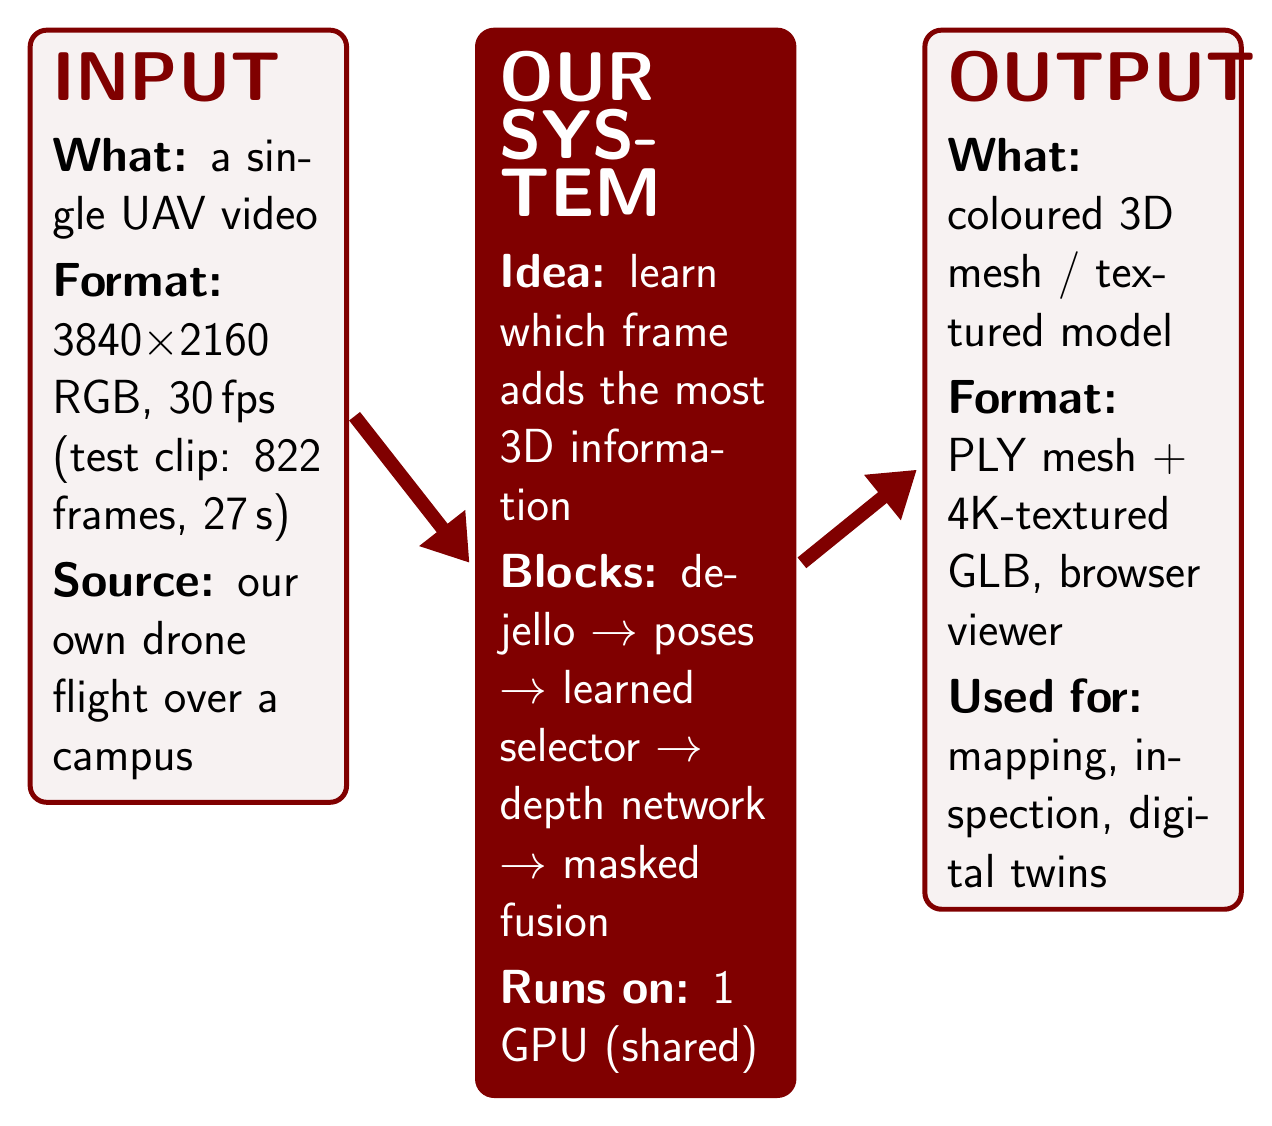
\begin{tikzpicture}[
    box/.style={draw=iitmaroon, line width=1.8pt, rounded corners=6pt,
      align=left, inner sep=8pt, minimum height=3.1cm, anchor=north west,
      font=\bodysize},
    arrow/.style={-{Triangle[length=16pt,width=20pt]}, line width=5pt, iitmaroon}]
  \node[box, fill=iitlight, text width=0.285\linewidth] (in) at (0,0)
    {{\headsize\bfseries\color{iitmaroon} INPUT}\\[0.3em]
     \textbf{What:} a single UAV video\\[0.2em]
     \textbf{Format:} 3840$\times$2160 RGB, 30\,fps (test clip: 822 frames, 27\,s)\\[0.2em]
     \textbf{Source:} our own drone flight over a campus};
  \node[box, fill=iitmaroon, text=white, text width=0.285\linewidth,
        right=1.6cm of in.north east, anchor=north west] (sys)
    {{\headsize\bfseries OUR SYSTEM}\\[0.3em]
     \textbf{Idea:} learn which frame adds the most 3D information\\[0.2em]
     \textbf{Blocks:} de-jello $\rightarrow$ poses $\rightarrow$ learned selector $\rightarrow$ depth network $\rightarrow$ masked fusion\\[0.2em]
     \textbf{Runs on:} 1 GPU (shared)};
  \node[box, fill=iitlight, text width=0.285\linewidth,
        right=1.6cm of sys.north east, anchor=north west] (out)
    {{\headsize\bfseries\color{iitmaroon} OUTPUT}\\[0.3em]
     \textbf{What:} coloured 3D mesh / textured model\\[0.2em]
     \textbf{Format:} PLY mesh + 4K-textured GLB, browser viewer\\[0.2em]
     \textbf{Used for:} mapping, inspection, digital twins};
  \draw[arrow] ([xshift=2pt]in.east) -- ([xshift=-2pt]sys.west);
  \draw[arrow] ([xshift=2pt]sys.east) -- ([xshift=-2pt]out.west);
\end{tikzpicture}
\end{posterblock}

% ======================== METHODOLOGY ========================
\begin{posterblock}{}{Proposed Methodology / System Architecture}
\centering
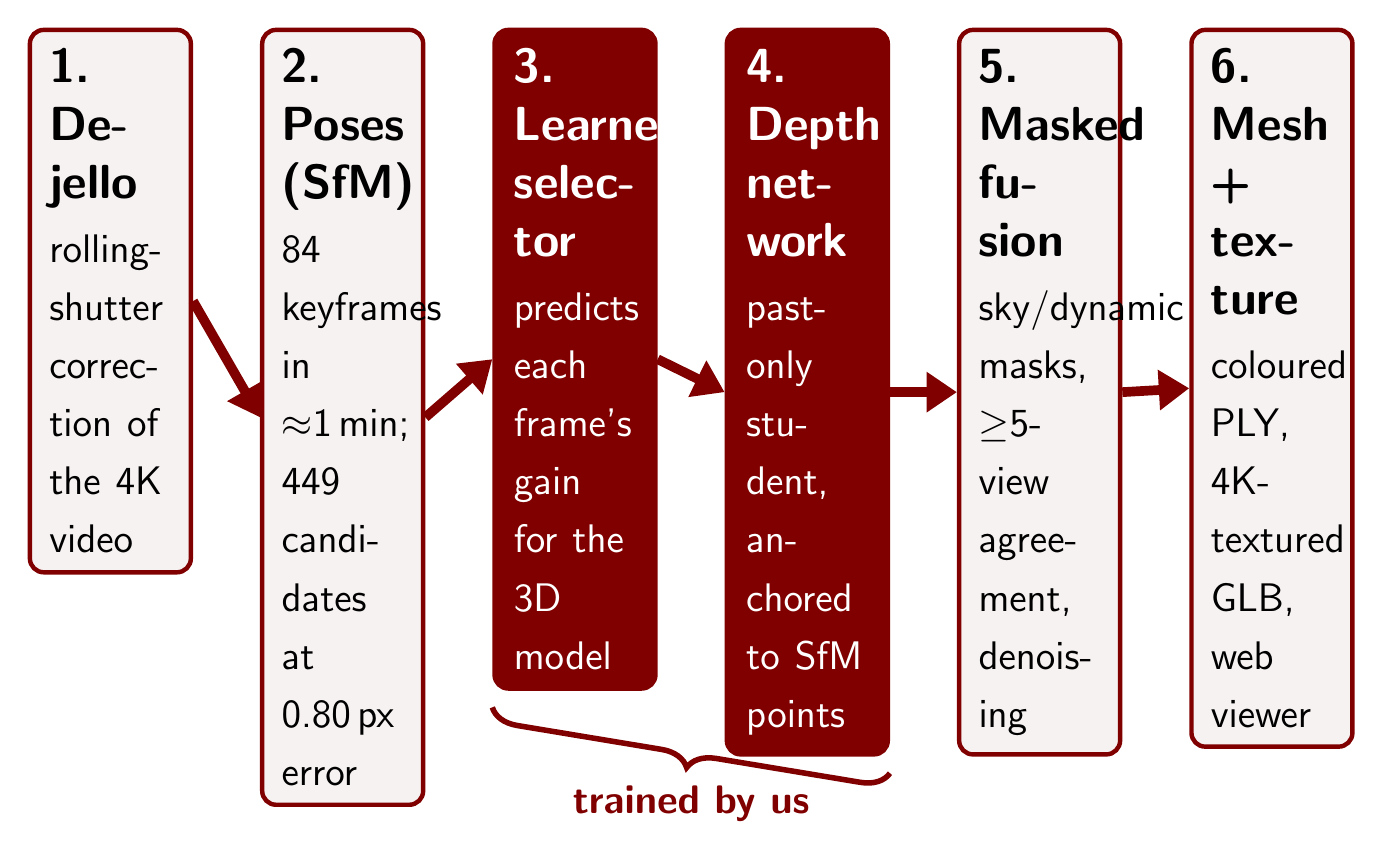
\begin{tikzpicture}[
    st/.style={draw=iitmaroon, line width=1.6pt, rounded corners=5pt, fill=iitlight,
      text width=0.128\linewidth, minimum height=3.3cm, align=left, inner sep=7pt,
      font=\bodysize, anchor=north west},
    ours/.style={st, fill=iitmaroon, text=white},
    ar/.style={-{Triangle[length=11pt,width=14pt]}, line width=3.5pt, iitmaroon}]
  \node[st] (a) at (0,0) {\textbf{1. De-jello}\\[2pt]{\smallsize rolling-shutter correction of the 4K video}};
  \node[st, right=0.85cm of a.north east, anchor=north west] (b) {\textbf{2. Poses (SfM)}\\[2pt]{\smallsize 84 keyframes in $\approx$1\,min; 449 candidates at 0.80\,px error}};
  \node[ours, right=0.85cm of b.north east, anchor=north west] (c) {\textbf{3. Learned selector}\\[2pt]{\smallsize predicts each frame's gain for the 3D model}};
  \node[ours, right=0.85cm of c.north east, anchor=north west] (d) {\textbf{4. Depth network}\\[2pt]{\smallsize past-only student, anchored to SfM points}};
  \node[st, right=0.85cm of d.north east, anchor=north west] (e) {\textbf{5. Masked fusion}\\[2pt]{\smallsize sky/dynamic masks, $\ge$5-view agreement, denoising}};
  \node[st, right=0.85cm of e.north east, anchor=north west] (f) {\textbf{6. Mesh + texture}\\[2pt]{\smallsize coloured PLY, 4K-textured GLB, web viewer}};
  \foreach \x/\y in {a/b,b/c,c/d,d/e,e/f} \draw[ar] (\x.east) -- (\y.west);
  \draw[decorate, decoration={brace, amplitude=10pt, mirror}, line width=2pt, iitmaroon]
    ([yshift=-6pt]c.south west) -- ([yshift=-6pt]d.south east)
    node[midway, below=12pt, font=\smallsize\bfseries, text=iitmaroon] {trained by us};
\end{tikzpicture}

\vspace{0.4em}
\raggedright
\begin{minipage}[t]{0.55\linewidth}\vspace{0pt}
\subhead{How the selector was trained}
\begin{enumerate}
  \item \textbf{Data:} 149,637 unique images from 9 datasets
    (JB3D 70k, UAVScenes 54k, Tanks\&Temples 13k, M3ED, NTU VIRAL, UAVLight, KITTI, Dronescapes, MatrixCity).
  \item \textbf{Counterfactual labels:} re-fuse the scene \emph{with} and \emph{without} each frame
    (our depth network) and record the F-score change against LiDAR-qualified geometry, also under
    blur, defocus and frame gaps: \textbf{258,573 training rows}.
  \item \textbf{Model:} ResNet18 image encoder (384-d) + 36-d map state $\rightarrow$ 4-layer Transformer with ADD/SWAP heads.
  \item \textbf{Training:} 28 epochs (185k steps) + expansion; the unseen AMtown03 flight picks the checkpoint.
\end{enumerate}
\end{minipage}%
\hfill
\begin{minipage}[t]{0.42\linewidth}\vspace{0pt}
\subhead{Objective and policy}
\[ \hat g(a) = f_\theta\big(\psi(I_{\text{cand}}),\, \psi(I_{\text{occ}}),\, s\big)
   \;\approx\; g(a) = F(\mathcal{S}\oplus a) - F(\mathcal{S}) \]
{\smallsize $\psi$: ResNet18 embedding; $s$: map state; $a$: ADD or SWAP; $\mathcal{S}$: kept frames; $F$: surface F-score.\par}
\vspace{0.3em}
Views are grouped into bins (DINO cosine $\ge 0.9$). \textbf{ADD} to an empty bin or \textbf{SWAP} its
occupant if $\hat g > \tau$; otherwise \textbf{KEEP}.\par
\vspace{0.3em}
\textbf{Combined mode:} rule keyframes give coverage; the selector picks the best frame near
each one (65 of 84 swapped) and adds 14 of its own.
\end{minipage}
\end{posterblock}

% ======================== QUALITATIVE ========================
\begin{posterblock}{}{Results on a Real Campus Flight (all rendered from the same viewpoint, no hand-editing)}
\begin{minipage}[t]{0.242\linewidth}\vspace{0pt}
  \tile{figures/fig_frame.jpg}{Input video frame}{De-jello 4K frame, $t=15.4$\,s.}
\end{minipage}\hfill
\begin{minipage}[t]{0.242\linewidth}\vspace{0pt}
  \tile{figures/fig_ref4k.jpg}{Reference: native-4K MVS}{84 frames at 3840\,px: \textbf{70.7\,min} dense, $\approx$\textbf{90\,min} textured.}
\end{minipage}\hfill
\begin{minipage}[t]{0.242\linewidth}\vspace{0pt}
  \tile{figures/fig_hybrid92.jpg}{Ours: combined (quality)}{92 frames, 2560\,px: \textbf{F = 0.98} vs reference.}
\end{minipage}\hfill
\begin{minipage}[t]{0.242\linewidth}\vspace{0pt}
  \tile{figures/fig_selected17.jpg}{Ours: 17 learned frames}{2\% of the video: \textbf{8.3\,min}, 97\% of surface.}
\end{minipage}
\end{posterblock}

% ======================== TWO FREE-FLOWING COLUMNS ========================
\begin{minipage}[t]{0.488\textwidth}\vspace{0pt}
% ---------- Results ----------
\begin{posterblock}{}{Results and Analysis}
\begin{keybox}
Same scene, same cameras: our learned-depth pipeline reaches F@2\% = 0.95
in \textbf{8.6\,min} vs \textbf{70.7\,min} for native-4K multi-view stereo (\textbf{8.2$\times$ faster}).
\end{keybox}
\centering
{\bodysize
\renewcommand{\arraystretch}{1.12}\setlength{\tabcolsep}{5pt}
\begin{tabular}{@{}lrrrr@{}}
  \toprule
  \textbf{Method} & \textbf{Frames} & \textbf{Time} & \textbf{F@1\%} & \textbf{F@2\%}\\
  \midrule
  Native-4K MVS (reference) & 84 & 70.7 / 90\,min$^\ast$ & -- & -- \\
  Ours, combined (quality) & 92 & 120\,min & \textbf{0.980} & \textbf{0.983}\\
  Ours, DA3 depth backbone & 84 & \textbf{8.6\,min} & 0.879 & 0.953\\
  Ours, depth student & 84 & 14.4\,min & 0.746 & 0.856\\
  Ours, learned 17 frames & 17 & \textbf{8.3\,min} & 0.726 & 0.796\\
  \bottomrule
\end{tabular}\par}
\vspace{4pt}\raggedright
{\smallsize\color{iitgray}F-score vs the 4K reference (threshold 1\% / 2\% of scene size, same cameras,
no alignment). Surface recall is 96--97\% for every learned-depth run. $^\ast$dense / textured.
All times on one GPU shared with another 20\,GB training job.\par}
\vspace{0.4em}
\subhead{Where the time goes} {\smallsize\color{iitgray}(minutes, same GPU)}\\[0.2em]
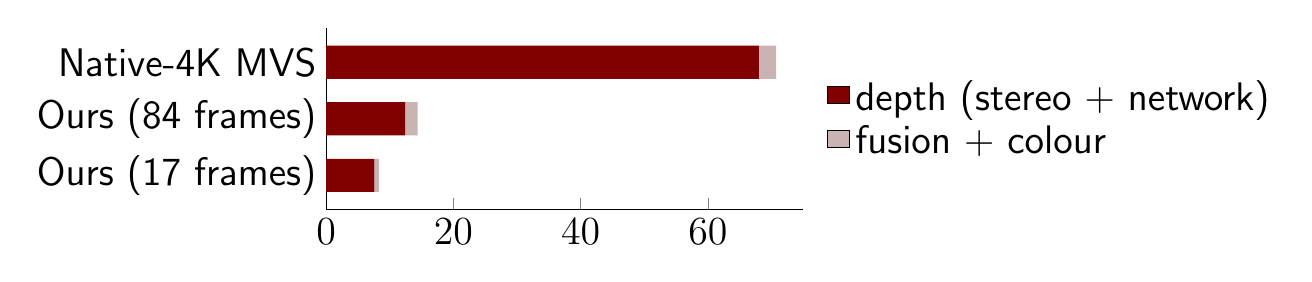
\begin{tikzpicture}
\begin{axis}[
  scale only axis, width=0.5\linewidth, height=2.3cm, xbar stacked, bar width=12pt,
  xmin=0, xmax=75, axis x line*=bottom, axis y line*=left,
  symbolic y coords={mvs,o84,o17},
  ytick=data, yticklabels={Native-4K MVS,Ours (84 frames),Ours (17 frames)}, y dir=reverse,
  enlarge y limits=0.3, tick label style={font=\smallsize},
  legend style={font=\smallsize, draw=none, at={(1.03,0.5)}, anchor=west, legend columns=1},
  legend cell align=left]
\addplot[fill=iitmaroon, draw=none] coordinates {(68,mvs) (12.4,o84) (7.6,o17)};
\addplot[fill=barlight, draw=none] coordinates {(2.7,mvs) (2.0,o84) (0.7,o17)};
\legend{depth (stereo + network), fusion + colour}
\end{axis}
\end{tikzpicture}
\end{posterblock}

% ---------- 4 ----------
\begin{posterblock}{4}{Toughest Problems We Solved}
\subhead{P1. No ground truth for ``a useful frame''}\\
\textbf{Solution:} counterfactual re-fusion labels under blur, defocus and frame-gap corruptions.
\textbf{Gain:} 258k training rows; AUC 0.74 on an unseen flight.

\vspace{0.2em}
\subhead{P2. Dense depth is the bottleneck}\\
\textbf{Problem:} 4K PatchMatch takes 68 of the 71 minutes.
\textbf{Solution:} a depth network anchored to sparse SfM points, fused with multi-view agreement.
\textbf{Gain:} 4.9--8.5$\times$ faster with 96--97\% of the surface recovered.

\vspace{0.2em}
\subhead{P3. Floating ``sky'' geometry}\\
\textbf{Solution:} each camera's sky mask votes out vertices it sees as sky.
\textbf{Gain:} 2--4\% noisy faces removed, buildings unchanged.
\end{posterblock}

% ---------- 7 ----------
\begin{posterblock}{7}{Key Learnings}
\begin{itemize}
  \item \textbf{Technical:} SfM/MVS, TSDF fusion, depth distillation, Transformers, 150k-image training.
  \item \textbf{Research:} a better label AUC does not guarantee a better 3D model; evaluate end to end.
  \item \textbf{Engineering:} resumable, timed pipelines on a shared GPU.
\end{itemize}
\end{posterblock}
\end{minipage}%
\hfill
\begin{minipage}[t]{0.488\textwidth}\vspace{0pt}
% ---------- 6 ----------
\begin{posterblock}{6}{Positioning vs Existing Work}
\centering
{\bodysize
\renewcommand{\arraystretch}{1.12}\setlength{\tabcolsep}{6pt}
\begin{tabular}{@{}lcccc@{}}
  \toprule
  \textbf{Capability} & \textbf{[1,2]} & \textbf{[3]} & \textbf{Uniform} & \textbf{Ours} \\
  \midrule
  Learns which frames help & \no & \no & \no & \yes \\
  Fast dense depth & \no & \yes & \partly & \yes \\
  Handles rolling-shutter jello & \no & \no & \no & \yes \\
  Removes sky / moving objects & \no & \no & \no & \yes \\
  Online (past-only) design & \no & \partly & \yes & \yes \\
  Time on our 27\,s clip & 71--90\,m & -- & -- & \textbf{8.3\,m} \\
  \bottomrule
\end{tabular}\par}
\vspace{4pt}\raggedright
{\smallsize\color{iitgray}\yes\ yes \ \partly\ partial \ \no\ no. [1,2] COLMAP SfM + PatchMatch MVS; [3] depth foundation model.\par}
\vspace{0.3em}
\textbf{Our position:} MVS treats every frame as equally useful; we \emph{learn} each frame's value for
the 3D model and pair the chosen frames with fast learned depth.

\vspace{0.4em}
\subhead{Frame selection on 100 held-out episodes}\\[0.2em]
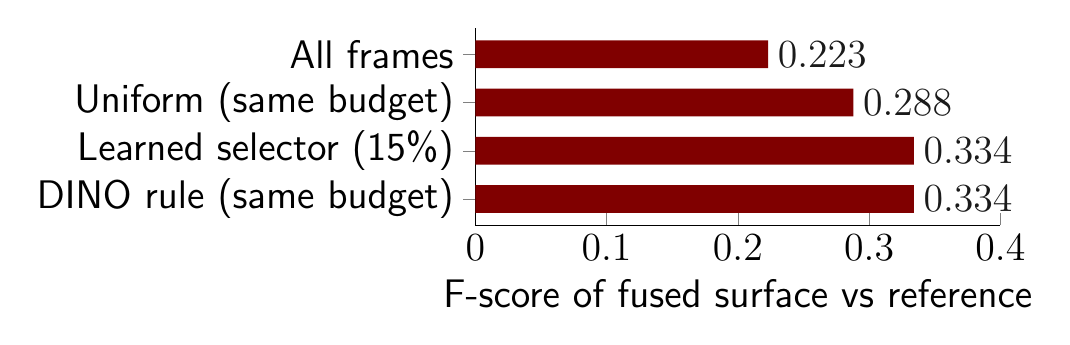
\begin{tikzpicture}
\begin{axis}[
  scale only axis, width=0.55\linewidth, height=2.5cm, xbar, bar width=10pt,
  xmin=0, xmax=0.4, xtick={0,0.1,0.2,0.3,0.4}, xticklabel style={/pgf/number format/fixed},
  axis x line*=bottom, axis y line*=left,
  symbolic y coords={all,uni,ours,dino},
  ytick=data, yticklabels={All frames,Uniform (same budget),Learned selector (15\%),DINO rule (same budget)},
  y dir=reverse, enlarge y limits=0.18,
  tick label style={font=\smallsize}, label style={font=\smallsize},
  xlabel={F-score of fused surface vs reference},
  nodes near coords, nodes near coords style={font=\smallsize\bfseries, anchor=west, text=iitdark, /pgf/number format/fixed, /pgf/number format/precision=3}]
\addplot[fill=iitmaroon, draw=none] coordinates {(0.223,all) (0.288,uni) (0.334,ours) (0.334,dino)};
\end{axis}
\end{tikzpicture}\par
\textbf{15\%} of frames chosen by the selector give a \textbf{50\% better} surface than all
frames and beat uniform sampling in 76\% of episodes (unseen flight: AUC 0.74). A tuned DINO
rule is equally strong, so we \textbf{combine} the two.
\end{posterblock}

% ---------- 5 ----------
\begin{posterblock}{5}{Critical Challenges Faced}
\begin{itemize}
  \item \textbf{Rolling-shutter ``jello''} in the 4K video broke SfM
        $\rightarrow$ de-jello correction before pose estimation.
  \item \textbf{Selector kept too few frames} (2\% of the video)
        $\rightarrow$ combined with rule keyframes for coverage.
  \item \textbf{Still open:} selector alone only ties a tuned DINO rule; quality mode is still slow.
\end{itemize}
\end{posterblock}

% ---------- Conclusion ----------
\begin{posterblock}{}{Conclusion and Future Work}
\begin{itemize}
  \item Learned frame selection + learned depth gives a near-reference 3D model of a
        real campus flight \textbf{5--8$\times$ faster} than native-4K MVS.
  \item \textbf{Next:} on-board online selection and a budget-aware policy.
\end{itemize}
{\smallsize
\subhead{References:}
[1] J.\,L. Sch\"onberger, J.-M. Frahm, ``Structure-from-Motion Revisited,'' \emph{CVPR}, 2016.\;
[2] J.\,L. Sch\"onberger \emph{et al.}, ``Pixelwise View Selection for Unstructured MVS,'' \emph{ECCV}, 2016.\;
[3] H. Lin \emph{et al.}, ``Depth Anything 3,'' \emph{arXiv}, 2025.\;
[4] M. Oquab \emph{et al.}, ``DINOv2,'' \emph{TMLR}, 2024.\par
\subhead{Acknowledgements:} Dr.\ Chalavadi Vishnu, Dept.\ of CSE, IIT Tirupati.\par}
\end{posterblock}
\end{minipage}

\vfill
\begin{tcolorbox}[enhanced, colback=iitmaroon, colframe=iitmaroon, arc=0pt,
  boxrule=0pt, left=16pt, right=16pt, top=7pt, bottom=7pt,
  fontupper=\affilsize\color{white}]
\textbf{M.Tech Project Poster Presentation 2026} \hfill
Indian Institute of Technology Tirupati
\end{tcolorbox}

\end{document}
